\chapter{Estrategia de resolución}

Este capítulo explica la estrategia de resolución seguida para resolver el problema de sincronización de semáforos en el Corredor Garzón. La metodología se basa en tres puntos: el modelado del problema, el algoritmo evolutivo desarrollado y el uso de técnicas de alto desempeño. El capitulo comienza presentando el modelado del problema, que incluye el diseño del mapa de la zona y la creación de instancias realistas que serán usadas para simular el tráfico en el simulador SUMO. En esta primera sección se presenta el simulador de tráfico SUMO y el trabajo de campo realizado para recabar datos precisos de la realidad. Luego el capítulo detalla el diseño e implementación del algoritmo evolutivo multiobjetivo, que fue desarrollado utilizando la biblioteca Malva. Finalmente se especifican los parámetros, características y modelo de paralelismo del Algoritmo Evolutivo implementado.


\section{Modelado del problema }

El modelado del problema comprende la simplificación de la realidad y el uso de aquellos elementos que resulten útiles para resolver el problema de sincronización de semáforos. El modelado se basa en el diseño de un mapa de la zona e instancias realistas que serán usadas en el simulador de tráfico SUMO. A continuación se presenta el simulador, las herramientas necesarias utilizadas y el proceso seguido para desarrollar el modelo. 

\subsection{Simulador SUMO (Simulation of Urban MObility)}

Como se explicó en el marco teórico, SUMO es un simulador de tráfico gratuito y de código abierto que permite modelar redes de calles, vehículos, transporte público, ciudadanos y semáforos. Este simulador sigue un modelo microscópico, ya que realiza la simulación individual explícita de cada elemento. SUMO incluye un conjunto de herramientas destinadas a facilitar la generación de tráfico y la construcción de mapas. 

Puesto que existe un amplio abanico de posibilidades a la hora de elegir un simulador de tráfico, se efectuó un análisis relacionado con las posibilidades y objetivos del proyecto. A continuación se presentan las razones que sustentan la elección de SUMO como el simulador de tráfico utilizado:

\begin{itemize}
	\item Portable: SUMO puede ser ejecutado tanto en Windows como en Linux. Esta característica es requerida, dado que Windows es una de las plataformas utilizadas para implementar el proyecto y Linux (CentOs) es el sistema operativo utilizada por el Cluster Fing donde se desarrolla el análisis experimental.
	
	\item Modos de ejecución: SUMO puede ejecutarse sin interfaz gráfica, utilizando solamente la línea de comando, lo que aumenta sensiblemente la velocidad de ejecución. Esta funcionalidad es fundamental a la hora de diseñar el algoritmo evolutivo, ya que la interacción con el simulador de tráfico debe ser eficiente. Por otro lado, presenta la opción de ejecutarse con interfaz gráfica, lo que es indispensable a la hora de visualizar la simulación. Esta opción es útil sobre todo en el inicio del desarrollo, cuando se realizan ajustes y pruebas.
	
	\item Gratuito y abierto: SUMO se presenta como un proyecto de código abierto y sin costo, siendo un factor importante para un proyecto de investigación como el que se quiere desarrollar. 
	
	\item Documentación y mantenimiento: Este simulador incluye una detallada documentación que hace más fácil su utilización. Cuenta con una comunidad muy activa que responde dudas en foros lo cual es útil a la hora de buscar soporte en caso de problemas u errores. SUMO también cuenta con un desarrollo activo que permite su mejora por medio de actualizaciones frecuentemente.
	
	\item Configuración simple: SUMO presenta un sencillo sistema de configuración, basada en archivos XML para la ejecución de las simulaciones. La modificación de estos archivos permiten alterar la configuración de los semáforos, las propiedades y rutas de los vehículos, entre otras opciones. Complementariamente cuenta con herramientas para importar mapas de servicios como \citet{OSM}.
	
	\item Información de salida: SUMO ofrece la opción de generar una amplía variedad de datos, producida por la simulación ejecutada. Entre estos datos se encuentran la velocidad de los vehículos y el largo del recorrido, datos que son requeridos por la solución propuesta.
	
	\item Eficiente: Soporta redes de tránsito muy grandes y está diseñado para ejecutar simulaciones a gran velocidad, siendo una característica deseable por la complejidad del problema a solucionar.
	
\end{itemize}


SUMO presenta un funcionamiento sencillo basado en tomar como entradas archivos de configuración que representan la red vial, los vehículos, el tráfico y los semáforos. Además, genera archivos de salida con información útil como el tiempo de simulación, la cantidad de vehículos, velocidad de los vehículos, duración del viaje, emisiones de gases contaminantes, etc. 

Dada la complejidad del problema a enfrentar, se utilizan otras herramientas para realizar ciertas tareas de manera más eficiente y con menos errores. \emph{NetConvert} viene integrado con SUMO y es utilizado para generar la red vial a partir del mapa obtenido de Open Street Map, transformándolo al formato que SUMO reconoce. Otra herramienta integrada con SUMO es \emph{DUaRouter} que permite generar recorridos de vehículos basado en dinámicas definidas por el usuario. \emph{Traffic Modeler} creado por \citet{TrafficModeler}, es útil para la generación de tráfico de manera visual que puede ser exportado al formato reconocido por SUMO. 
	


\begin{figure}[H]
	\centering
	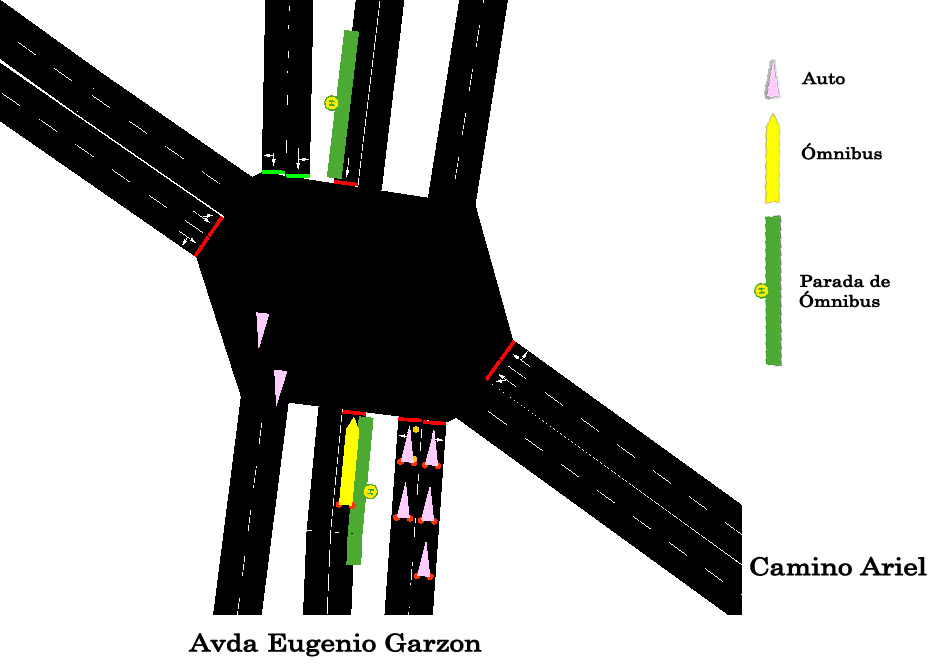
\includegraphics[width=0.9\linewidth]{Figures/sim1}
	\caption[Simulación de trafico en el simulador SUMO.]{Simulación de tráfico en el simulador SUMO en el cruce entre Bulevar Battle y Ordoñez y el Corredor Garzón.}
	\label{fig:sim1}
\end{figure}



\subsection{Proceso de modelado}

El objetivo del proceso de modelado es el desarrollo de instancias realistas del problema. Se comienza con el diseño del mapa que representa la zona del Corredor Garzón. Luego se describe el trabajo de campo realizado para obtener datos precisos de la realidad. Finalmente utilizando estos datos, se describe el desarrollo de las instancias realistas que serán utilizadas en el simulador de tráfico.

\subsubsection{Diseño del mapa}

El primer paso del modelado consiste en desarrollar un mapa de la zona del Corredor Garzón que sea compatible con el simulador. Se utiliza el servicio de Open Street Map \citep{OSM} que cuenta con mapas libres y actualizados por una comunidad muy activa. Se importa la zona de interés del mapa al editor JOSM(Java OpenStreetMap Editor) para poder adecuarlo a las necesidades del problema.  Se utilizaron otros servicios (Google Maps y Bing Maps) y un estudio de la zona para validar la correctitud del mapa importado desde OSM. Se detectaron inconsistencias entre la realidad y el mapa que fueron corregidas, por ejemplo en la dirección de las rutas y el diseño de algunos cruces.  

El alcance geográfico comprende al Corredor Garzón en toda su extensión y dos caminos paralelos a cada lado del mismo.
Como se ve en el mapa de la figura \ref{fig:mapa_osm_sumo}, no existen calles paralelas reales, por lo que el proceso para diseñar el mapa consistió en: seleccionar las calles que construyen dos caminos paralelos a cada lado del Corredor Garzón, luego, seleccionar las calles internas entre las paralelas. Se verifica que cada camino paralelo incluya calles doble mano o dos calles de una sola mano, finalmente se borran las demás calles que no están incluidas en la zona modelada.


Dado los cambios realizados en el mapa, como la eliminación de calles que no formaban parte de la zona modelada, no se pudo contribuir con la comunidad OSM subiendo el mapa con las modificaciones que corregían algunas inconsistencias encontradas.



\begin{figure}[H]
	\centering
	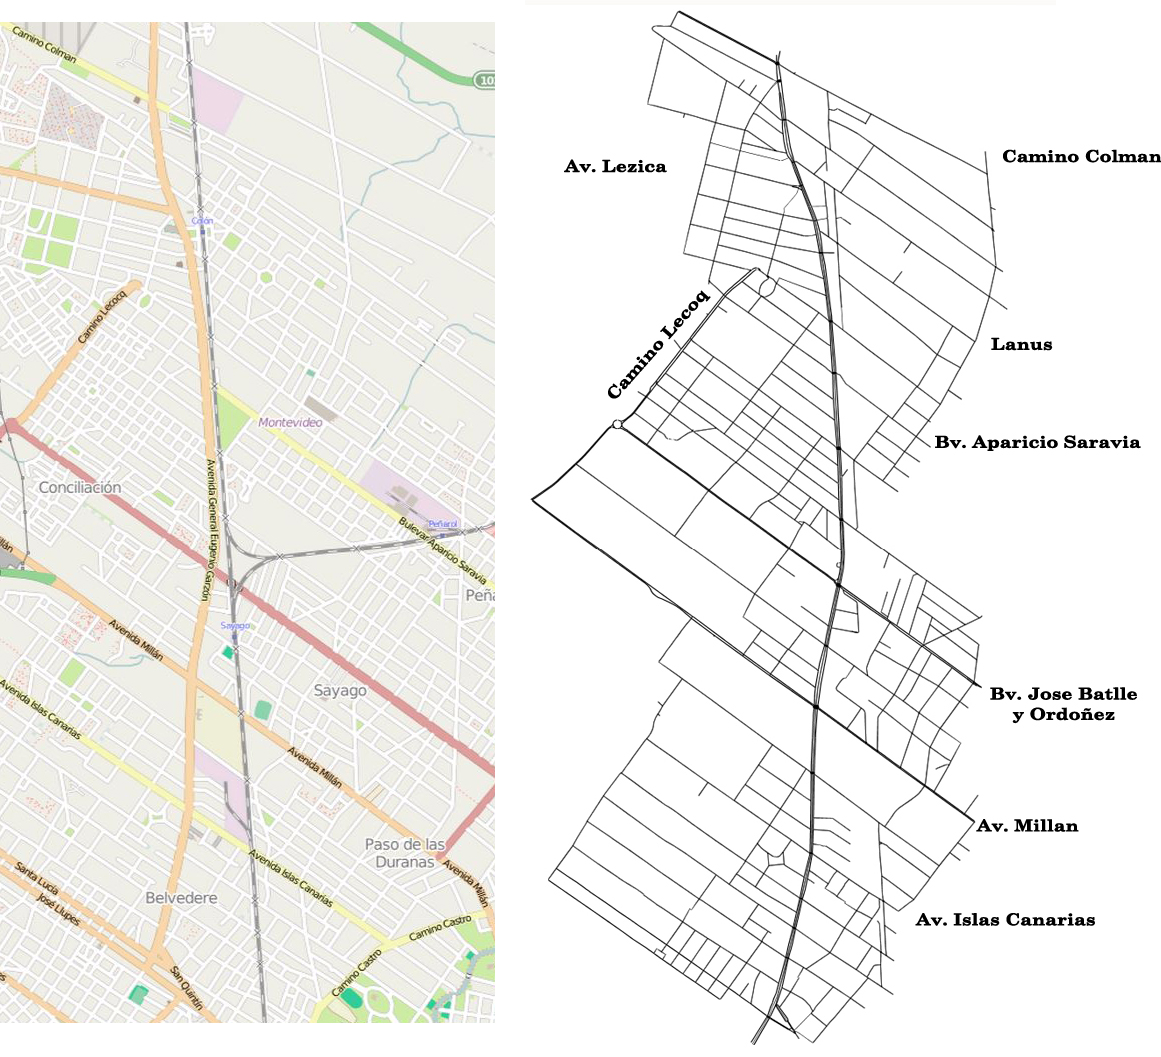
\includegraphics[width=0.9\linewidth]{Figures/mapa_osm_sumo}
	\caption[Mapa del corredor Garzón]{Mapa del corredor Garzón. A la izquierda el mapa extraído de OSM, a la derecha el mapa procesado listo para ser usado en SUMO. El corredor Garzón está en el centro de cada imagen.}
	\label{fig:mapa_osm_sumo}
\end{figure}

La herramienta \emph{Netconvert} fue utilizada para transformar el mapa obtenido desde OSM, al formato XML que reconoce el simulador SUMO. Esta herramienta no reconoce algunos datos incluidos en el formato OSM, por ejemplo: los números de las casas, vías de tren, vías de peatones, caminos, plazas, paradas y los separadores que tiene el corredor de las vías para autos, entre otros. Se destaca como punto importante que NetConvert no reconoce correctamente a los corredores, ya que confunde y superpone el corredor central con las vías para los autos, seguramente por no reconocer los separadores físicos que presenta el corredor. Para solucionar este problema se utilizó el programa JOSM para eliminar los datos no reconocidos por NetConvert y editar el mapa, separando aproximadamente un metro las calles del corredor central. Esta modificación permitió que NetConvert interpretara correctamente el funcionamiento del corredor, para que los vehículos no se trasladaran entre la vía de los autos y la del corredor de ómnibus. Pero este cambio implementado generó un problema, ya que cada cruce de la realidad pasó a ser representado por tres cruces distintos (uno por cada calle del corredor). Para solucionar el problema anterior y otros errores, se realizaron ajustes manuales, modificando los archivos xml relacionados. Entre otros cambios, se especificó manualmente las reglas de movilidad correctas en algunos cruces, por ejemplo cuando estaba prohibido virar a la izquierda.

Al finalizar el proceso de diseño, se obtuvo un mapa fiel a la realidad, delimitado en la zona del Corredor Garzón que es compatible con el simulador de tráfico SUMO.


\subsubsection{Trabajo de campo}

Existen datos públicos disponibles sobre la cantidad de ómnibus y sus frecuencias, pero no se tienen datos sobre la densidad del tráfico vehicular en la zona del Corredor Garzón. Por este motivo se realizó un revelamiento in-situ en cinco cruces representativos. Los cruces seleccionados fueron: Camino Ariel, Battle y Ordoñez, Plaza Videla, Camino Colman y Aparicio Saravia. Estos cruces presentan diferentes características que son útiles para modelar variantes en la cantidad de vehículos circulantes. 

Se siguieron las recomendaciones de los textos consultados relacionados con el conteo vehicular \citep{ConteoTrafico}. El día seleccionado para efectuar el conteo fué el miércoles, con clima soleado y en el horario de 15:00 a 17:00 horas, para no obtener sesgos que se producen los fines de semana, en horas pico, o en días de lluvia. Se realizaron filmaciones de entre 15 y 30 minutos en los cruces y luego se analizaron los vídeos para efectuar el conteo manual con la posibilidad de enlentecer el vídeo para mayor facilidad. Luego se completó una planilla electrónica (figura \ref{fig:conteo_hoja}) donde se incluyen: la cantidad de vehículos que recorren el Corredor Garzón, los que circulan por la calle que cruza y los que doblan. 

\begin{figure}[H]
	\centering
	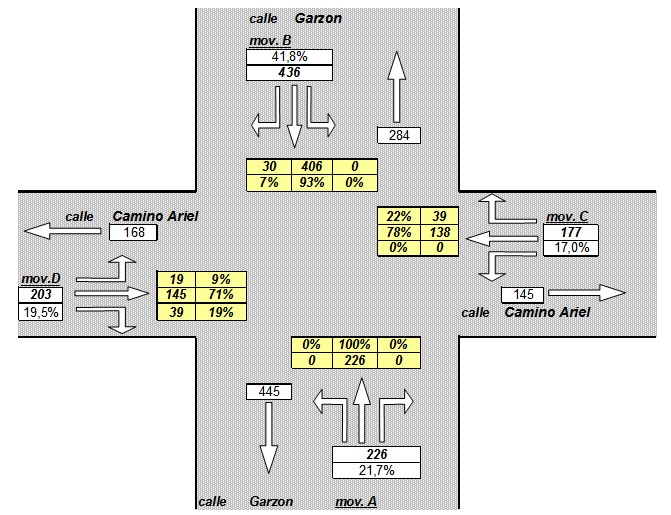
\includegraphics[width=0.9\linewidth]{Figures/conteo_hoja}
	\caption[Ejemplo de planilla electrónica para el conteo manual de tráfico.]{Ejemplo de planilla electrónica para el conteo manual de tráfico en la intersección entre el corredor Garzón y Camino Ariel}
	\label{fig:conteo_hoja}
\end{figure}



\begin{table}[H]
	\renewcommand{\arraystretch}{1.2}
	\caption[Resumen del revelamiento del tráfico en la zona del corredor Garzón.]{Resumen del revelamiento del tráfico en la zona del corredor Garzón. Se muestra la cantidad de vehículos y la orientación hacia donde circulan.}
	\label{table:resumen_trafico}
	\centering
	\begin{tabular}{lcccc}
		\hline
		Intersección&
		Sur-Garzón& 
		Norte-Garzón & 
		Oeste &
		Este 
		\\ 
		\hline
		Camino Colman  & 410 & 390 & 140 & 230\\		
		Plaza Vidiella  & 400 & 444 & 292 & 0\\		
		Aparicio Saravia  & 390 & 450 & 40 & 90\\		
		Battle y Ordoñez  & 510 & 390 & 470 & 300 \\	
		Camino Ariel  & 436 & 226 & 177 & 203 \\													
		\hline
		
		
		\hline
	\end{tabular}
\end{table}

La tabla \ref{table:resumen_trafico} muestra la cantidad de vehículos en los distintos cruces; hay que tener en cuenta que solamente se contabilizan los autos, no se tienen en cuenta otro tipo de vehículos.

Se realizaron recorridas de punta a punta del corredor a una velocidad constante en auto para ser utilizados como datos a la hora de desarrollar las simulaciones de tráfico. Con este análisis se obtiene tanto la duración total del recorrido, como el tiempo que permanece detenido en los cruces semaforizados. 

Para la configuración de los semáforos, se realizó un recorrido en bicicleta por toda la extensión del Corredor Garzón. Se cronometró la duración de las luces de los semáforos en cada esquina recorriendo el camino de ida, y para validar los tiempos también se relevaron las duraciones de las luces en el camino de vuelta. Estos tiempos fueron verificados por los vídeos obtenidos anteriormente en el conteo del tráfico.


\subsubsection{Desarrollo de instancias realistas del problema}

Una vez completado el diseño del mapa compatible con el simulador de la zona del Corredor Garzón,  y obtenidos los datos relevados de la realidad, se procede al desarrollo de instancias realistas que representen la situación actual en relación con el tráfico.

Existen varios modelos disponibles para representar la circulación de los vehículos. El modelo \emph{aleatorio} genera diferentes recorridos aleatorios que seguirán los vehículos. En el modelo \emph{basado en áreas} se especifican diferentes áreas que indican los lugares donde el tráfico se origina y donde finaliza. Un modelo más complejo es el \emph{basado en actividad} donde se definen la cantidad de casas, vehículos y población de una zona determinada. Luego el modelo genera la densidad de tráfico basado en los tipos de actividades que se realizan comúnmente, como ir al trabajo, hacer las compras, ir a la escuela, etc. Finalmente un modelo muy utilizado, sobre todo en escenarios de tamaño reducido, es el \emph{definido por el usuario} que permiten determinar la ruta de cada vehículo con mayor detalle.

Se utilizó el programa Traffic Modeler \citep{TrafficModeler} que se caracteriza por generar modelos de tráfico complejos de manera visual. Se optó por un modelo de movilidad entre áreas, lo que permite una buena granularidad al especificar la densidad de tráfico. El programa genera el recorrido del viaje para cada vehículo, que se mantienen constantes en las distintas ejecuciones del algoritmo evolutivo. La variación se produce en las velocidades desarrolladas por cada uno, ya que dependiendo de la configuración de los semáforos logrará mayores o menores velocidades.



\begin{figure}[h]
	\centering
	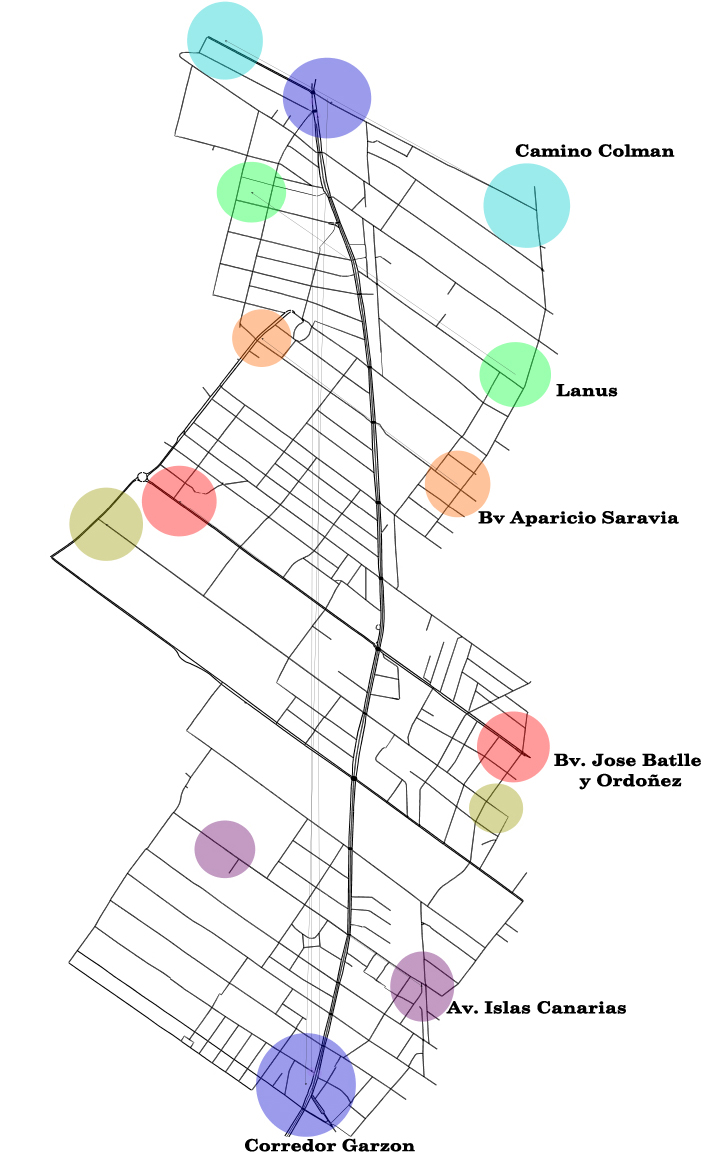
\includegraphics[width=0.5\linewidth]{Figures/areaflow1}
	\caption[Mapa diseñado en el TrafficModeler para la generación de tráfico.]{Mapa diseñado en el TrafficModeler para la generación de trafico. Los círculos del mismo color especifican el tráfico entre esas áreas. }
	\label{fig:areaflow1}
\end{figure}


Se plantea el uso de dos tipos de vehículos: autos y ómnibus. Cada tipo de vehículo posee diferentes características asociadas, como el tamaño, aceleración y velocidad máxima. No se especifican otros tipos de vehículos como motos o camiones ya que el trabajo se enfoca en los dos primeros tipos. Se agregaron las frecuencias y los distintos recorridos de los ómnibus obtenidos de datos públicos de la Intendencia Municipal de Montevideo(IMM). Las frecuencias incluyen las líneas urbanas: 'G', '409' ,'2', 'd5'  y  '148'. Las líneas de ómnibus suburbanas realizan  un mismo  trayecto las cuales no van a ser tomadas en cuenta en la optimización del algoritmo pero si aparecerán en la simulación.

La ubicación y líneas de cada parada se obtuvo del Servicio de Información Geográfica de Montevideo (http://sig.montevideo.gub.uy). Existen 14 paradas de líneas urbanas por el Corredor Garzón para el recorrido de ida y la misma cantidad para la vuelta. Se realizaron variantes en los recorridos dentro de una misma línea para simular el hecho de que no siempre se detienen en las mismas paradas. Se tuvo en cuenta el tiempo que demora un ómnibus al detenerse en una parada y que existen paradas donde por la cantidad de pasajeros se demora más tiempo. La duración de la detención en las paradas fueron obtenidas en el lugar, con tiempos de entre 15 a 35 segundos.

Se realizó un estudio basado en datos de GPS proporcionados por la IMM. Estos datos cuentan con la posición exacta, la velocidad instantánea y la referencia del ómnibus, para un conjunto de líneas seleccionadas tomadas en un período de una semana. 
Para este procesamiento se utilizó QGIS, un sistema de información geográfico capaz de visualizar, editar y realizar operaciones sobre elementos geográficos. Adicionalmente fue necesario el desarrollo de \emph{scripts} para obtener las estadísticas necesarias, ya que la cantidad de información estudiada era muy grande (1.5Gb). El uso de QGIS permitió seleccionar, filtrar y relacionar los datos de posición y velocidad con las líneas que circulan por el Corredor Garzón. Luego de procesar los datos se constató una velocidad media de 14.5 km/h en el Corredor Garzón lo que permitió ajustar mejor el modelo. 

Para configurar la simulación del tráfico se utilizan como entrada tres archivos de configuración en formato XML que son reconocidos por el simulador SUMO. El primero, es el archivo de \emph{configuración de los semáforos} donde se detalla la duración de las luces, el comienzo de fase y la ubicación de los mismos en el mapa base. El segundo archivo representa la \emph{ruta de los vehículos} que contiene el recorrido de cada vehículo. Finalmente el archivo con el \emph{recorrido de los ómnibus} indica el recorrido de los mismos, su frecuencia, la ubicación de las paradas, en cuales se detienen y cuanto demoran en la parada.

Finalizando este proceso se cuenta con todos los elementos necesarios para la creación de instancias realistas del problema que serán utilizadas en el simulador para modelar la realidad. En el próximo capitulo donde se desarrolla el análisis experimental se describen los escenarios que hacen uso de estas instancias modificando algunas variables como la densidad del trafico para ajustarlo a las necesidades de la experimentación.


%REDACTAR: no me convence mucho el titulo
\section{Arquitectura de la solución}

El esquema de la figura \ref{fig:arquitectura1}  muestra la arquitectura propuesta para el problema. La biblioteca Malva se utiliza para la implementación del algoritmo evolutivo. En cada evaluación de la función de fitness se realiza un llamado al simulador SUMO. El primer paso consiste en generar la población inicial del algoritmo evolutivo, estos individuos representan una la configuración de semáforos para todo el Corredor Garzón, que incluye la duración de las fases y el \emph{offset}. Luego por cada individuo se genera un archivo compatible con el simulador que representa la configuración de semáforos. Este archivo se utiliza como entrada para ejecutar el simulador para cada individuo. Al finalizar la ejecución se generan archivos de salida que son procesados por el algoritmo evolutivo. Los datos de salida incluyen información necesaria para calcular el \emph{fitness} de cada individuo como la velocidad media de ómnibus y otros vehículos. El algoritmo se detiene al alcanzar un número de generaciones determinado, en ese momento se crea un archivo con la mejor configuración de semáforos encontrada. 

\begin{figure}[H]
	\centering
	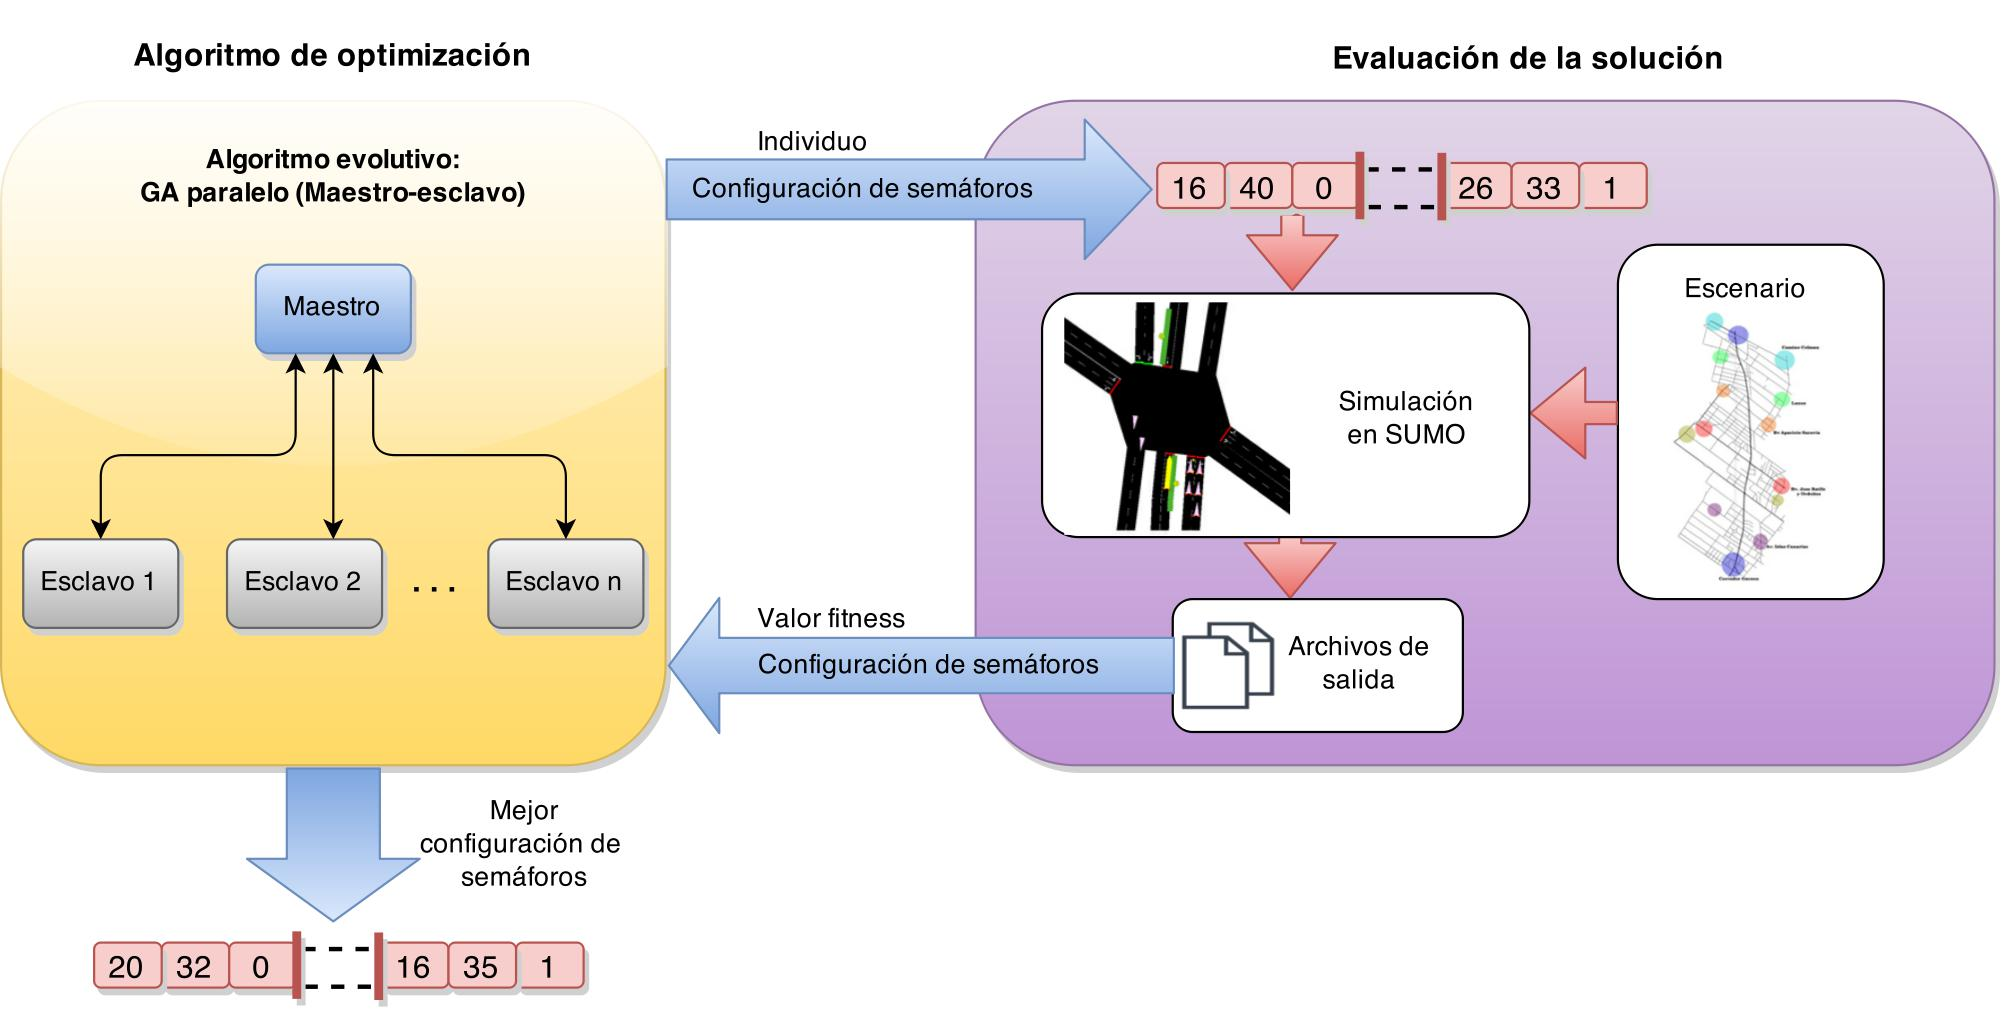
\includegraphics[width=0.7\linewidth]{Figures/arquitectura1}
	\caption{Arquitectura de la función de fitness}
	\label{fig:arquitectura1}
\end{figure}


\section{Implementación: Biblioteca Malva}

Dada la complejidad del problema, se contempló desde el inicio del proyecto la utilización de un \emph{framework} para el desarrollo del algoritmo evolutivo, de esta forma, se logra una ejecución eficiente y una implementación robusta pero flexible. 

Como se detalló en el marco teórico, existen varias opciones disponibles para seleccionar un \emph{framework}. Por las particularidades del problema planteado, existen ciertos requerimientos a la hora de seleccionar un \emph{framework}, entre los que se destacan:

\begin{itemize}
	\item Código abierto y gratuito: Al ser un proyecto de investigación de índole académico es conveniente que no se tengan costos económicos asociados. Además, es importante que se cuente con el código abierto con el fin de introducir modificaciones en el código base o corregir errores.
	\item Algoritmo genético: El \emph{framework} debe facilitar el desarrollo de un algoritmo genético ya que es la base en la que se sustenta el proyecto.
	\item Algoritmo paralelo: Por la complejidad del problema y el alto consumo de recursos computacionales que insume, es fundamental que incluya la opción de ejecución en paralelo. Si no cuenta con funcionalidad nativa, al menos que exista la posibilidad de modificar el código base para agregarlo.
	\item Plataforma: Es requerido que se pueda ejecutar en el Cluster Fing (CentOs - Linux), en Windows y otros sistemas Linux, ya que son las plataformas en donde se desarrolla y donde se realiza el análisis experimental del trabajo.
	\item Confiabilidad: Es deseable que el \emph{framework} sea lo suficientemente estable como para tener confianza de que el algoritmo funcionará de manera correcta. Por ejemplo que existan casos de éxito usando el \emph{framework}, documentación, ejemplos de código, etc.
	\item Lenguaje: Es deseable que esté desarrollado en C++ o Java por la experiencia que se cuenta en estos lenguajes. 
	\item Multiobjetivo: Es deseable (aunque no requerido) que soporte algoritmos multiobjetivo, ya que la función que se quiere implementar aún siendo multiobjetivo es sencilla.	
\end{itemize} 

Luego de analizar los puntos anteriores, se selecciona la biblioteca Malva para la implementación del algoritmo evolutivo. A continuación se detalla su funcionamiento y características.

Como se explicó anteriormente, \citet{Malva} surge como una variante del proyecto \citet{Mallba}. Propone su actualización, mejora y desarrollo como un proyecto de código abierto colaborativo.  Su objetivo es proveer de varios esqueletos de heurísticas de optimización que puedan ser utilizados y extendidos de manera fácil y eficiente. Los esqueletos se basan en separar dos conceptos: El problema concreto que se quiere resolver y por otro lado el método utilizado para resolverlo. Por tanto un esqueleto se puede ver como una instancia de una plantilla genérica para resolver un problema particular, manteniendo todas las funcionalidades genéricas.

Malva utiliza el lenguaje C++, con el objetivo de brindar modularidad y flexibilidad. Los esqueletos se ofrecen como un conjunto de clases requeridas que el usuario deberá modificar para adaptarlo a su problema, y las provistas que incluyen todos los aspectos internos del esqueleto siendo  independientes del problema particular. Entre los algoritmos provistos se encuentra el de Algoritmos genéticos y \citet{CHC}.


\section{Especificación del Algoritmo Genético utilizado}
Se utiliza el algoritmo genético provisto por la biblioteca  Malva llamado NewGA con las modificaciones detalladas en la sección anterior. El siguiente esquema describe el funcionamiento del algoritmo utilizado:

\begin{algorithm}[H]
	\caption{Algoritmo Genético de Malva. }
	\label{alg:algoritmo_genetico_malva}
	\begin{algorithmic} [1] 
		{
			\STATE \texttt{t} = 0
			\STATE {Inicializo( P(t))}
			\STATE {Evaluar estructuras en ( P(t))}			
			\WHILE {\text{No termine}}
			\STATE \texttt{t}++		
			\STATE {Seleccionar C(t) de P(t-1)}	
			\STATE {Recombinar estructuras en C(t) formando C'(t)}				
			\STATE {Mutar estructuras en C'(t) formando C''(t)}		
			\STATE {Evaluar estructuras en C''(t) generando un hilo de ejecucion por cada una}					
			\STATE {Consolidar valores de la evaluacion}								
			\STATE {Reemplazar P(t) de C''(t) y P(t-1)}								
			\ENDWHILE
		}
	\end{algorithmic}
	
\end{algorithm}

A continuación se realiza un resumen de las características del algoritmo implementado, que en la siguiente sección serán tratados detalladamente:
\begin{itemize}

\item Algoritmo paralelo: Utiliza el método maestro-esclavo donde en cada iteración el maestro genera un hilo por cada ejecución  de la función \emph{fitness} y luego espera a la terminación de todos los hilos para consolidar los datos. 
\item Función Multiobjetivo: Se intenta optimizar tanto la velocidad promedio de vehículos como la de ómnibus, teniendo cada uno un peso específico.
\item Representación del cromosoma: Es un vector de números naturales que representan la duración de las fases de los semáforos y el \emph{offset} para todos los semáforos del Corredor Garzón.
\item Cruzamiento y mutación: Se implementa una variante del cruzamiento de un punto específico para este problema y se utilizan dos tipos de mutación para modificar la duración de fase y el \emph{offset} de los semáforos.
\item Selección y reemplazo: Reemplaza padres por hijos. La selección de los padres se realiza por el método de torneo de tres individuos y la selección de hijos por el método de ruleta.

\end{itemize}

\subsection{Representación del cromosoma}

Como se explicó en el marco teórico, el problema de sincronización de semáforos puede ser resuelto optimizando diferentes parámetros. Entre estos parámetros se encuentran la duración de fase, de ciclo y el \emph{offset}. Dependiendo de cuáles se seleccionen deberán ser incluidos en la representación del cromosoma.

Para la solución propuesta se contempla tanto la duración de fase como el \emph{offset}. El cromosoma se agrupa lógicamente en cruces, siendo el valor de cada gen la duración de una
fase en un cruce, además se agrega para cada cruce el valor del \emph{offset}. Se utiliza un vector de números naturales para favorecer la claridad en el desarrollo y la facilidad a la hora de aplicar los operadores. Por este motivo el tamaño del cromosoma depende de la cantidad de cruces y de la cantidad de fases que incluya cada cruce. Con esta representación se busca una optimización global de todo el sistema y no individualmente para cada cruce, lo cual es fundamental para mejorar la velocidad promedio del Corredor Garzón y del resto de las calles que lo cruzan.

En la representación del cromosoma se omiten las luces amarillas ya que no modifican los tiempos reales del paso de vehículos.
 
 \begin{figure}[h]
 	\centering
 	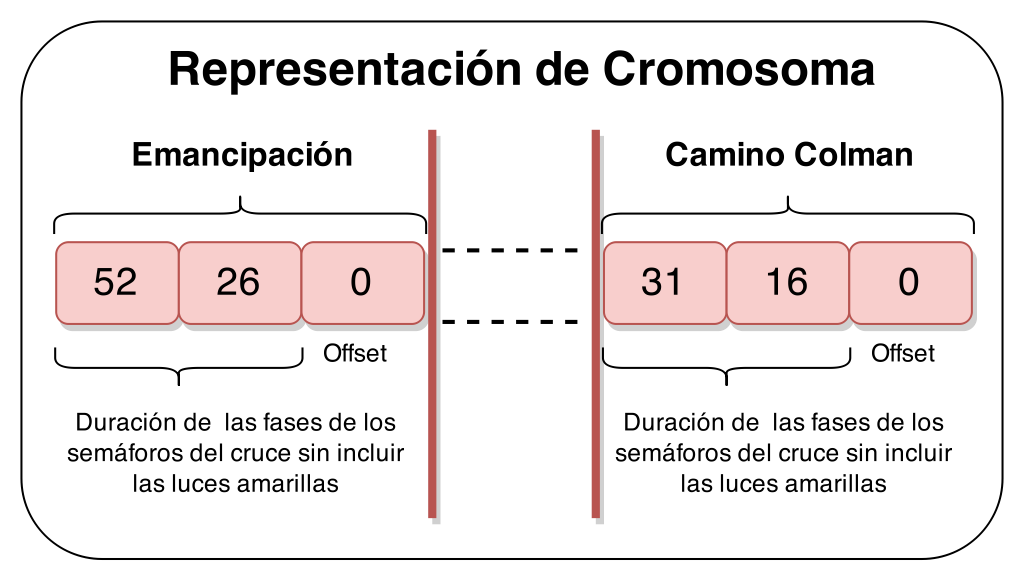
\includegraphics[width=0.7\linewidth]{Figures/cromosoma1}
 	\caption{Cromosoma de dos cruces}
 	\label{fig:cromosoma1}
 \end{figure}
 
Es importante que el algoritmo evolutivo genere solamente soluciones factibles, por lo tanto se tiene especial cuidado al ejecutar los operadores de cruzamiento y mutación.

\begin{figure}[H]
	\centering
	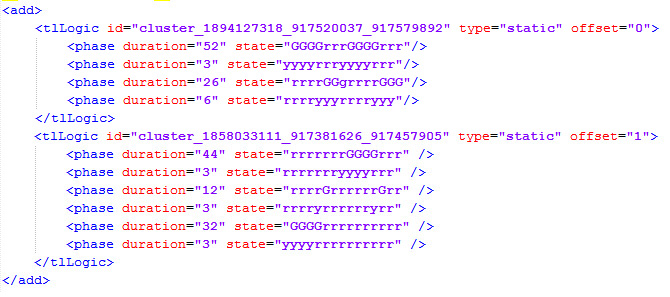
\includegraphics[width=\linewidth]{Figures/rep_sumo2}
	\caption{Representación de Sumo}
	\label{fig:rep_sumo}
\end{figure}

La figura \ref{fig:rep_sumo} muestra el archivo de configuración de semáforos que utiliza el simulador SUMO para el cromosoma anterior, donde se representan las fases. Por ejemplo la fase \emph{GGGGrrrGGGGrrr} indica la secuencia de luces y su duración de 52 segundos, \emph{G} indica la luz verde, \emph{r} la roja, \emph{y} el Amarillo. El valor del \emph{offset} indica el inicio de la fase. 

La figura \ref{fig:sem_numerados} presenta la numeración de los semáforos que se corresponden con la primera fase de este ejemplo, donde cada posición de la secuencia \emph{estado} se corresponde con un color en particular. 

\newpage
Por tanto para el estado \emph{GGGGrrrGGGGrrr} se tiene que:
\begin{itemize}
\item GGGG se corresponde a 1, 2, 3 y 4. 
\item rrr a 5, 6 y 7. 
\item GGGG a 8, 9, 10 y 11. 
\item rrr a 12, 13 y 14. 
\end{itemize}
  
\begin{figure}[H]
	\centering
	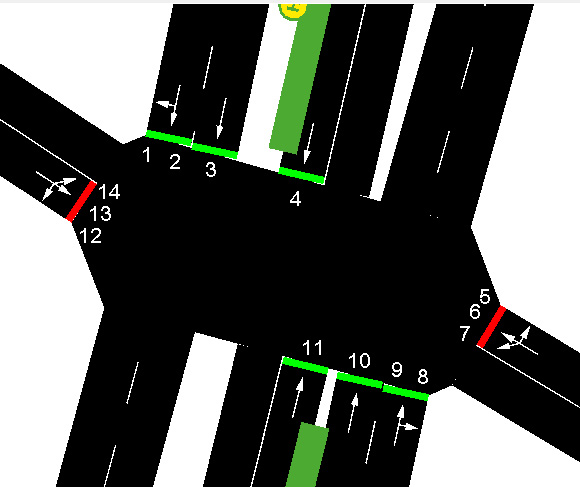
\includegraphics[width=0.7\linewidth]{Figures/semaforos_numerado}
	\caption[Representación de una fase de los semáforos para un cruce.]{Representación de una fase de los semáforos para un cruce. Cada número se corresponde a una letra en la secuencia de \emph{state} del archivo de configuración del simulador SUMO.}
	\label{fig:sem_numerados}
\end{figure}

\subsection{Población inicial}

Para la inicialización de la población se toma como referencia
la configuración obtenida a partir de los datos de la realidad,  luego para cada cruce se varían las duraciones de las fases de manera aleatoria entre un rango de valores configurable. Además se selecciona la fase inicial aleatoriamente entre la cantidad de fases del cruce.

\subsection{Función \emph{fitness}}


La evaluación de un individuo se realiza generando un archivo con la configuración de los semáforos en base a su cromosoma y ejecutando el simulador SUMO utilizando esta configuración para obtener los datos necesarios para calcular el \emph{fitness}.

Se emplea una función multiobjetivo usando combinación lineal de la velocidad de los ómnibus y del resto de los vehículos, ya que es un método sencillo y adecuado cuando son menos de tres objetivos. El \emph{fitness} se calcula como una suma ponderada, con los pesos fijados a priori.

        \begin{equation}
        \label{eq:funcion_fitness_generica}
		F(x) = \sum_{i=1}^{n}{w_i}{f_i}(x)
        \end{equation}

Se selecciona como objetivo la velocidad promedio de los ómnibus (vpb) y la velocidad promedio del resto de los vehículos (vpv). Esta métrica fue elegida pues es más adecuada para realizar las comparaciones con la realidad. Por ejemplo la cantidad de vehículos que completan su viaje, la duración promedio del recorrido o el tiempo de simulación son todas métricas que podrían usarse pero no son útiles a la hora de realizar comparaciones con la realidad.

La siguiente es la fórmula de \emph{fitness} utilizada, donde \emph{x} e \emph{y} indican los pesos que se especifican en la función. En una primera instancia se establece x = y = 1, más adelante se experimentará con otros pesos.

        \begin{equation}
        \label{eq:funcion_fitness}
        f = x.vpb + y.vpv
        \end{equation}
        


Se plantea optimizar la velocidad promedio de los vehículos en toda la red vial, de manera global, esto quiere decir que se busca una mejor velocidad promedio tanto en autos que van por Garzón como aquellos que circulan por los cruces o calles paralelas. La optimización global es fundamental, ya que si cada cruce se optimiza individualmente podría generar problemas de congestión en otras zonas.

\subsection{Operadores}
\subsubsection{Operador de Cruzamiento}
Se utiliza cruzamiento de un punto, seleccionando del cromosoma una posición aleatoria entre dos cruces como punto de corte, por tanto si un tramo del corredor tiene un buen comportamiento se intenta mantener esa propiedad. En el escenario que plantea la siguiente figura, los padres cuentan con tres cruces. Se elige un punto de corte aleatoriamente entre dos cruces y se generan los hijos que son una combinación de los padres.

\begin{figure}[H]
	\centering
	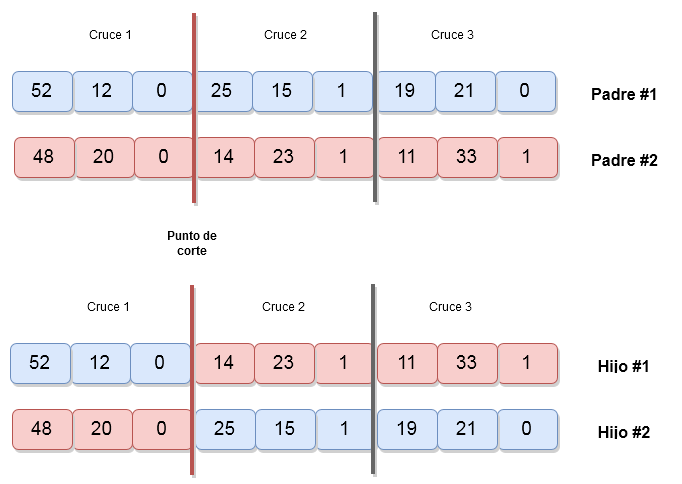
\includegraphics[width=8cm]{Figures/alg_cruzamiento}
	\caption{Visualización del cruzamiento entre individuos.}
	\label{fig:op_cruzamiento}
\end{figure}



\subsubsection{Operador de Mutación}
Se implementaron dos tipos de mutación:
\begin{itemize}

\item Mutación de duración de fase: para cada fase de cada cruce se modifica su duración sumando o restando una cantidad dada de segundos, con una probabilidad dada. Teniendo en cuenta que el valor obtenido se encuentre dentro de un rango especificado para que no se produzcan casos irreales como un cruce de menos de 5 segundos.

\item Mutación del \emph{offset}: Se elige aleatoriamente una fase con la cual va a comenzar el cruce con una probabilidad dada.
\end{itemize}

\subsubsection{Operador de selección y reemplazo}
Se  utilizan los operadores provistos por el algoritmo genético newGA de Malva. La selección de padres se realiza por el método de torneo de tres individuos y la selección de hijos por el método de ruleta. La política de reemplazo indica que tanto padres como hijos pueden ser parte de la siguiente generación (no solamente los hijos), por lo que existe reemplazo de padres por hijos.

\subsubsection{Parámetros del algoritmo}
Los parámetros específicos del algoritmo se establecen en el siguiente capítulo, donde se realiza un análisis experimental para encontrar los más adecuados. Estos parámetros son: número de generaciones, tamaño de población, probabilidad de cruzamiento y de mutación.


\section{Modelo de paralelismo e implementación}

Uno de los requisitos planteados al inicio del presente trabajo era la creación de un algoritmo genético que soportara paralelismo, con el objetivo de reducir los tiempos de ejecución. El motivo principal fue que los escenarios planteados se consideraron complejos y que utilizarían gran cantidad de recursos computacionales. Para este propósito, se utilizó como código base el algoritmo genético provisto por la biblioteca Malva llamado NewGA. A dicho código se le realizaron algunas modificaciones para lograr su ejecución en paralelo. Específicamente se modificó la forma en que se evalúan los individuos, generando un hilo de ejecución por cada individuo y distribuyendo la evaluación.

Se utilizó el método maestro-esclavo para el modelo de paralelismo. El proceso maestro se encarga de la mayoría de las etapas del algoritmo evolutivo, al comenzar, inicializa la población y se encarga de distribuir la evaluación de los individuos hacia los esclavos, creando un hilo de ejecución por cada esclavo. Luego el proceso maestro espera a que las evaluaciones terminen para obtener los valores de \emph{fitness} de los esclavos. Una vez obtenidos los valores, selecciona a los mejores individuos y le aplica los operadores de cruzamiento y mutación. Para finalizar ejecuta el operador de reemplazo para generar la siguiente población. Mientras, los esclavos se encargan solamente de obtener el individuo enviado por el maestro y de efectuar la evaluación del individuo, que corresponde a ejecutar el simulador y obtener los datos de salida.

En el capitulo siguiente, en la sección de análisis experimental se realiza un estudio de la eficiencia computacional del algoritmo genético paralelo, para comparar los tiempos de ejecución entre la versión paralela y en serie.